\documentclass[sigconf,review,anonymous]{acmart}

\usepackage{amsmath}
\usepackage{algorithm}
\usepackage{algpseudocode}
\usepackage{booktabs}
\usepackage{placeins}
\usepackage{subcaption}
\usepackage{tikz}
\usetikzlibrary{arrows.meta,calc,fit,positioning}

\settopmatter{printacmref=true}
\renewcommand\footnotetextcopyrightpermission[1]{}

\acmConference[SoCC '26]{ACM Symposium on Cloud Computing}{November 18--20, 2026}{Singapore}
\acmYear{2026}
\copyrightyear{2026}

\title{Guarded First-Decodable-Time Scheduling for Sparse Flexible Coded Learning in Cloud-Native Worker Services}
\subtitle{Research Full Paper}

\begin{document}

\begin{abstract}
Heterogeneous cloud workers make synchronous distributed learning vulnerable to
long-tail iteration latency.  Sparse flexible codes reduce redundant work, but
they still leave a systems question open: which recoverable row set becomes
visible first at runtime.  We present \textsc{G-port} (Guarded Prefix-Oriented
Runtime), a worker-service controller whose coded arm keeps the
sparse-flexible code fixed while changing the runtime order in which
recoverable row sets are exposed.  It combines
target-specific row scores, worker speed and delay estimates, deadline-aware
matching, exact online decodability checks, and a fixed guard that enables the
adaptive arm only when predicted prefix savings exceed overhead; otherwise it
falls back to static sparse-flexible placement.  We evaluate \textsc{G-port}
with trace-driven simulation and worker-service
prototypes, including TCP, network-stressed TCP, and a direct three-node K3s
deployment.  Across the worker-service evaluation, \textsc{G-port} improves
barrier latency by up to 24.8\% in deployed K3s stress tests, remains positive
across all main TCP, network-stressed TCP, and K3s scale points, and maintains
bounded recovery under communication, interference, cancellation, and
worker-close stress.  These
results show that row-exposure order is a practical scheduling lever inside
fixed coded-computing deployments.
\end{abstract}


\begin{CCSXML}
<ccs2012>
   <concept>
       <concept_id>10003033.10003079.10003080</concept_id>
       <concept_desc>Networks~Cloud computing</concept_desc>
       <concept_significance>500</concept_significance>
   </concept>
   <concept>
       <concept_id>10010520.10010521.10010537</concept_id>
       <concept_desc>Computer systems organization~Distributed architectures</concept_desc>
       <concept_significance>300</concept_significance>
   </concept>
   <concept>
       <concept_id>10010147.10010257.10010258.10010259</concept_id>
       <concept_desc>Computing methodologies~Distributed computing methodologies</concept_desc>
       <concept_significance>300</concept_significance>
   </concept>
</ccs2012>
\end{CCSXML}

\ccsdesc[500]{Networks~Cloud computing}
\ccsdesc[300]{Computer systems organization~Distributed architectures}
\ccsdesc[300]{Computing methodologies~Distributed computing methodologies}

\keywords{coded computing, distributed learning, straggler mitigation, cloud scheduling}

\maketitle

\section{Introduction}

Cloud platforms increasingly run distributed learning jobs on heterogeneous
and shared clusters.  Worker speeds, queueing delays, network variability, and
co-located interference create long-tail iteration times.  Tail-at-scale
analysis showed that a small fraction of slow components can dominate service
latency~\cite{dean2013tail}.  Cluster systems turned the same observation into
runtime mechanisms: speculative execution mitigates slow MapReduce tasks
\cite{zaharia2008late}, Mantri diagnoses and reacts to outliers in
MapReduce clusters~\cite{ananthanarayanan2010mantri}, and Dolly uses cloning to
reduce straggler impact~\cite{ananthanarayanan2013dolly}.  These systems
established a useful design principle: the scheduler should optimize the unit
that actually gates completion, not just the average work issued to the
cluster.  For synchronous distributed learning, that gate is revisited at every
iteration, so even modest worker-speed mismatch can repeatedly become a
barrier-latency problem.

Modern ML cluster schedulers apply this principle at the job and training-stack
layers.  Optimus models the marginal value of resources for distributed deep
learning jobs~\cite{peng2018optimus}.  Gandiva exploits introspection to
time-slice and pack deep learning workloads~\cite{xiao2018gandiva}.  Tiresias
schedules GPU jobs with learned job progress information~\cite{gu2019tiresias}.
Themis studies fair and efficient GPU sharing~\cite{mahajan2020themis}.  Gavel
makes heterogeneity an explicit cluster-scheduling dimension
\cite{narayanan2020gavel}.  Pollux co-adapts training batch size and cluster
allocation for goodput~\cite{qiao2021pollux}.  Sia extends goodput
optimization to heterogeneous ML clusters~\cite{subramanya2023sia}.  Recent
systems continue the same trajectory: RLTune combines learned prioritization
with solver-based allocation~\cite{dongare2025rltune}; Cuckoo optimizes
deadline-aware GPU job packing~\cite{zhang2025cuckoo}; Sailor automates
distributed training over dynamic heterogeneous clusters~\cite{strati2025sailor};
What-if analysis diagnoses training stragglers~\cite{lin2025whatifstragglers};
Holmes localizes irregularities in large GPU fleets~\cite{yao2025holmes};
Minder detects faulty machines during large-scale training~\cite{deng2025minder};
GREYHOUND targets fail-slow behavior in hybrid-parallel training
\cite{wu2025greyhound}; and Zeppelin balances variable-length LLM training
work~\cite{chen2026zeppelin}.  The common abstraction in these systems is that
heterogeneity is managed through job priority, resource allocation, packing,
placement, or diagnosis.  That abstraction is powerful, but it does not expose
the algebraic dependency among encoded rows inside a coded iteration.

Coded computing changes the completion condition of an iteration.  Gradient
coding uses algebraic redundancy so that a master can recover a full gradient
without waiting for every worker~\cite{tandon2017gradient}.  Short-Dot reduces
the cost of coded linear transforms through sparse coded products
\cite{dutta2016shortdot}.  Coded distributed learning generalizes this idea to
machine-learning iterations~\cite{lee2018speeding}.  Sparse coded matrix
multiplication further reduces coded-linear-algebra overhead
\cite{wang2018codedsparse}.  Approximate gradient coding studies heterogeneous
stragglers under relaxed recovery~\cite{song2025approxgc}.  Sparse flexible
coded learning (SFCL) creates the closest exact baseline for this paper: a
fixed sparse-flexible code matrix with multiple legal recovery
paths~\cite{zhang2025sparseflexible}.
These constructions move the barrier from ``all assigned work is complete'' to
``some algebraically sufficient row set is complete.''  This shift creates a
runtime question that code construction alone does not answer: among many legal
recovery paths, which one will become visible first under the current worker
speeds, dispatch delays, cancellation behavior, and sparse row costs.

The resulting scheduling problem is neither ordinary load balancing nor
general cluster placement.  In sparse flexible coded learning, the code defines
a row-span family rather than a single required worker set
\cite{zhang2025sparseflexible}.  An encoded row is useful only when it arrives
with other completed rows whose span contains the target gradient.  A
cost-balanced runtime can therefore place expensive sparse rows on fast workers
and still delay the first decodable row set, because row cost and row
decodability measure different things.  A generic heterogeneity-aware runtime
can also miss the same signal: cluster schedulers such as Gavel expose
heterogeneity as a job-to-resource placement problem~\cite{narayanan2020gavel},
whereas coded learning needs a row-prefix objective inside one iteration.  This
observation gives the background for our method.  The scheduler should preserve
the fixed
sparse-flexible code, predict how a candidate assignment changes the
first-decodable prefix, and enable adaptation only when the predicted prefix
reduction is large enough to pay for scheduling, extra-work, communication, and
cancellation overhead.

We present \textsc{G-port}, a guarded worker-service controller for sparse
flexible coded learning.  The name abbreviates Guarded Prefix-Oriented
Runtime: the controller keeps the code fixed and changes which row prefix is
exposed first.  Its coded arm assigns a target-specific importance score to
encoded rows, aggregates scores over row pairs, maps decode-critical pairs to
workers predicted to finish early, and runs the same row-span test as the
decoder to predict the first-decodable prefix.  A fixed online guard
enables the adaptive arm only when worker-speed mismatch, predicted
first-decode gain, prefix growth, and
rows-after-decode counters pass; otherwise \textsc{G-port} falls back to static
sparse-flexible placement.  The design keeps the
sparse-flexible code fixed and focuses on the worker-service runtime that
controls row exposure order.  Coded-only and alternative-fallback variants are
treated as ablations, not separate proposed systems.

The paper makes four contributions.

\begin{itemize}
  \item We identify first-decodable row exposure as a systems objective for
  sparse flexible coded learning.  The objective asks the runtime to expose an
  algebraically sufficient row prefix early, while leaving the code
  construction and decoder unchanged.
  \item We design \textsc{G-port}, a guarded worker-service controller with
  decode-aware row scores, finish-time estimates, first-prefix prediction, and
  static sparse-flexible fallback.  A fixed online guard enables the adaptive
  coded arm only when the predicted prefix reduction is worth its runtime cost.
  \item We specify the deployment semantics that make the design safe to use:
  reassignment changes row-to-worker order but not the recoverable row-span
  family, decoding is accepted only by the exact row-span test, and guard
  decisions are made before each iteration rather than after observing the
  outcome.
  \item We evaluate the design against scheduler-style baselines using
  trace-driven simulation and worker-service prototypes, including a direct
  three-node K3s deployment.  Across the main TCP, network-stressed TCP, and
  K3s worker-service comparisons, \textsc{G-port} remains positive at all tested
  worker counts; its bounded reissue path restores decode success under a
  single worker-close stress.
\end{itemize}

\section{Background and Motivation}

\subsection{Coded Distributed Learning}

In synchronous distributed learning, the training data are split into
$m$ shards and the master coordinates one gradient computation at iteration
$t$.  Let $w_t$ be the current model and let $g_j(w_t)$ denote the partial
gradient computed from shard $j$.  The full gradient is
\begin{equation}
  \label{eq:full-gradient}
  g(w_t) = \sum_{j=1}^{m} g_j(w_t),
\end{equation}
so an uncoded synchronous system must wait until every shard contribution has
arrived.  Gradient coding~\cite{tandon2017gradient} and related coded
computation methods~\cite{lee2018speeding} avoid this all-worker wait by
asking workers to compute encoded linear combinations of shard gradients.  The
master then reconstructs the same vector $g(w_t)$ after receiving a sufficient
subset of encoded results.

\subsection{Sparse Flexible Coded Computing}

Sparse flexible coded learning constructs a code matrix by stacking two sparse
row blocks
\begin{equation}
  \label{eq:sfcl-code}
  B =
  \begin{bmatrix}
    A^{(1)} \\
    A^{(2)}
\end{bmatrix}
  \in \mathbb{R}^{2n \times m},
\end{equation}
where $n$ is the number of workers and $m$ is the number of data shards.  The
matrix in Equation~\eqref{eq:sfcl-code} has one column per shard and $2n$
encoded rows.  Let $b_r^\top$ be row $r$ of $B$; the coefficient $b_{rj}$ says
how shard $j$ participates in encoded row $r$.  A zero coefficient means that
row $r$ does not touch shard $j$, which is where sparsity reduces arithmetic
work.  Let
$G_t=[g_1(w_t),\ldots,g_m(w_t)]^\top$ denote the stack of shard gradients at
iteration $t$.  Encoded row $r$ computes the vector
\begin{equation}
  \label{eq:encoded-row}
  \tilde{g}_r = b_r^\top G_t = \sum_{j=1}^{m} b_{rj} g_j(w_t).
\end{equation}
Equation~\eqref{eq:encoded-row} uses $b_r^\top G_t$ as shorthand for the
weighted vector sum on the right-hand side.  Let
$S \subseteq \{1,\ldots,2n\}$ be the indexes of encoded rows that have
completed and returned to the master.  Define
$B_S \in \mathbb{R}^{|S|\times m}$ as the submatrix of $B$ formed by selecting
the completed rows in $S$.  The master can decode once
\begin{equation}
  \label{eq:decode-span}
  \mathbf{1}_m \in \mathrm{span}(B_S^\top).
\end{equation}
Here $\mathbf{1}_m$ is the all-ones vector of length $m$, because recovering the
full gradient in Equation~\eqref{eq:full-gradient} requires coefficient one on
every shard gradient.
The notation $\mathrm{span}(B_S^\top)$ denotes the column span of
$B_S^\top$, equivalently all linear combinations of the completed row
coefficient vectors.  Thus Equation~\eqref{eq:decode-span} says that the
completed rows can be linearly combined to produce the all-ones coefficient
vector.  Equivalently, there exists a decoding vector
$c_S \in \mathbb{R}^{|S|}$ such that
\begin{equation}
  \label{eq:decode-vector}
  B_S^\top c_S = \mathbf{1}_m.
\end{equation}
Multiplying the received encoded gradients by the same coefficients $c_S$
recovers the uncoded full gradient $g(w_t)$.

Decodability is decoder-dependent.  Equations~\eqref{eq:decode-span}
and~\eqref{eq:decode-vector} describe exact linear decoding, as implemented by
a rank or Gaussian-elimination-style solve.  A peeling or BP decoder would use a
different success predicate based on whether iterative singleton recovery can
finish.  Such a predicate can be stricter than the span condition: a returned
row set may be linearly sufficient for Gaussian decoding but not peelable by
BP.  This paper uses the exact row-span predicate throughout; BP-aware
first-decodable scheduling is a natural extension with a different decoder
predicate.

The sparse flexible construction mainly decides which rows exist and how sparse
they are.  In a cloud system, the runtime must also decide which row pair goes
to which worker.  This paper focuses on that runtime degree of freedom.

\subsection{Cost-Only Assignment Failure}
\label{sec:motivation}

Sparse encoded rows have different arithmetic costs because they touch
different numbers of nonzero data blocks.  A cost-aware scheduler assigns
expensive rows to fast workers.  This can reduce total completed computation
time, but the first decodable set may depend on rows that are not locally most
expensive.  If such rows are delayed, the master still waits even though many
other rows have finished.

Figure~\ref{fig:motivation} illustrates this gap with one iteration of a fixed
code.  The code already makes the pair $\{r_2,r_5\}$ a legal recovery set.  A
cost-aware order sorts work by local row cost and worker speed, without asking
which rows jointly make the target decodable; in the example, it exposes
$r_3$ and $r_6$ before both recovery rows have arrived.  A decode-aware order
instead tries to expose a legal recovery set early; here, it places $r_2$ and
$r_5$ in the first two completions.  The runtime gap is therefore the
difference between the first decodable times, not a difference in code
construction.  The guard enables adaptive placement only when the predicted
prefix reduction is large enough to dominate scheduling, extra-work,
communication, and cancellation costs.

\begin{figure}[t]
  \centering
  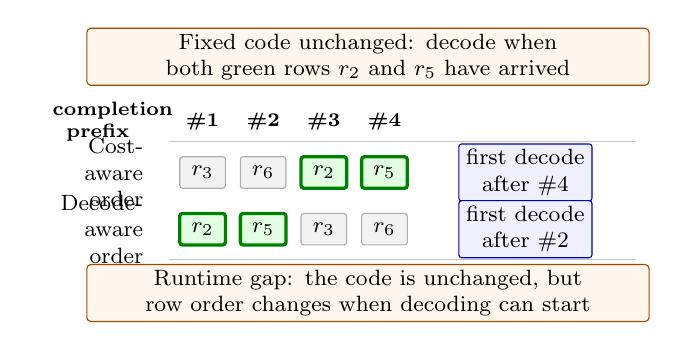
\begin{tikzpicture}[
      font=\footnotesize,
      row/.style={draw, rounded corners=1pt, align=center,
        minimum width=0.58cm, minimum height=0.40cm, inner sep=1pt},
      crit/.style={row, fill=green!11, draw=green!50!black, very thick},
      other/.style={row, fill=gray!10, draw=gray!65},
      marker/.style={draw=blue!70!black, fill=blue!6, rounded corners=1pt,
        align=center, inner sep=2pt, text width=1.55cm},
      note/.style={draw, rounded corners=1.5pt, align=center, inner sep=2pt,
        fill=orange!7, draw=orange!60!black},
      head/.style={font=\scriptsize\bfseries, align=center},
      sep/.style={gray!45, line width=0.25pt}
    ]
    \node[note, text width=7.0cm] at (3.45,0)
      {Fixed code unchanged: decode when both green rows $r_2$ and $r_5$ have arrived};

    \node[head, anchor=east, text width=1.15cm] at (0.72,-0.82) {completion\\prefix};
    \node[head] at (1.35,-0.82) {\#1};
    \node[head] at (2.12,-0.82) {\#2};
    \node[head] at (2.89,-0.82) {\#3};
    \node[head] at (3.66,-0.82) {\#4};
    \draw[sep] (0.92,-1.07) -- (6.85,-1.07);

    \node[anchor=east, align=right, text width=1.35cm] at (0.72,-1.47)
      {Cost-aware\\order};
    \node[other] (c1) at (1.35,-1.47) {$r_3$};
    \node[other] (c2) at (2.12,-1.47) {$r_6$};
    \node[crit]  (c3) at (2.89,-1.47) {$r_2$};
    \node[crit]  (c4) at (3.66,-1.47) {$r_5$};
    \node[marker] (cd) at (5.45,-1.47) {first decode\\after \#4};

    \node[anchor=east, align=right, text width=1.35cm] at (0.72,-2.19)
      {Decode-aware\\order};
    \node[crit]  (f1) at (1.35,-2.19) {$r_2$};
    \node[crit]  (f2) at (2.12,-2.19) {$r_5$};
    \node[other] (f3) at (2.89,-2.19) {$r_3$};
    \node[other] (f4) at (3.66,-2.19) {$r_6$};
    \node[marker] (fd) at (5.45,-2.19) {first decode\\after \#2};

    \draw[sep] (0.92,-2.57) -- (6.85,-2.57);
    \node[note, text width=7.0cm] at (3.45,-3.00)
      {Runtime gap: the code is unchanged, but row order changes when decoding can start};
  \end{tikzpicture}
  \caption{Row completion order changes the first-decodable prefix even when
  the code is fixed.}
  \Description{A timeline-style example. The same fixed code allows rows r2
  and r5 to decode. Under cost-aware order, two other rows finish first and
  decoding happens at prefix four. Under decode-aware order, r2 and r5
  finish first and decoding happens at prefix two.}
  \label{fig:motivation}
\end{figure}

We verify the effect in Figure~\ref{fig:motivation} with a deliberately small
mechanism diagnostic before introducing the design.  The diagnostic fixes an
8-worker/8-shard sparse-flexible code, generates five code instances, samples
12 worker-state rounds per instance, and changes only the row-pair priority
used to expose rows.  For each round, it predicts row completion times from
sparse row costs and sampled worker speeds, then runs the same row-span check
after each completion to find the first-decodable prefix.  Static placement has
31.6 ms predicted mean first-decode time.  A cost-only priority improves the
mean to 25.4 ms, but still needs 9.1 completed rows on average before decode.
An oracle decode-priority order, computed by enumerating minimal decodable
subsets in this tiny code, reaches 19.3 ms and reduces the first-decodable
prefix by 1.2 rows relative to static placement.  The oracle is not a deployable
scheduler, and the diagnostic does not include network or service overhead; it
isolates the reason Figure~\ref{fig:motivation} matters.  The design below
therefore uses cheap decodability-aware row scores and an online guard rather
than treating row cost alone as the scheduling objective.

\section{Design}
\label{sec:design}

Figure~\ref{fig:architecture} summarizes the system boundary.  The sparse
flexible code matrix is fixed before an iteration, so the runtime does not
change which encoded rows or recovery sets exist.  \textsc{G-port} operates on
the worker-service path: it scores row pairs, predicts whether an adaptive
assignment will expose a decodable prefix earlier than static placement, runs a
fixed online guard, and then streams rows to TCP or K3s worker services.  The
exact row-span decoder remains the correctness gate, while the observed
first-decode event feeds the guard counters for later rounds.

\begin{figure*}[tbp]
  \centering
  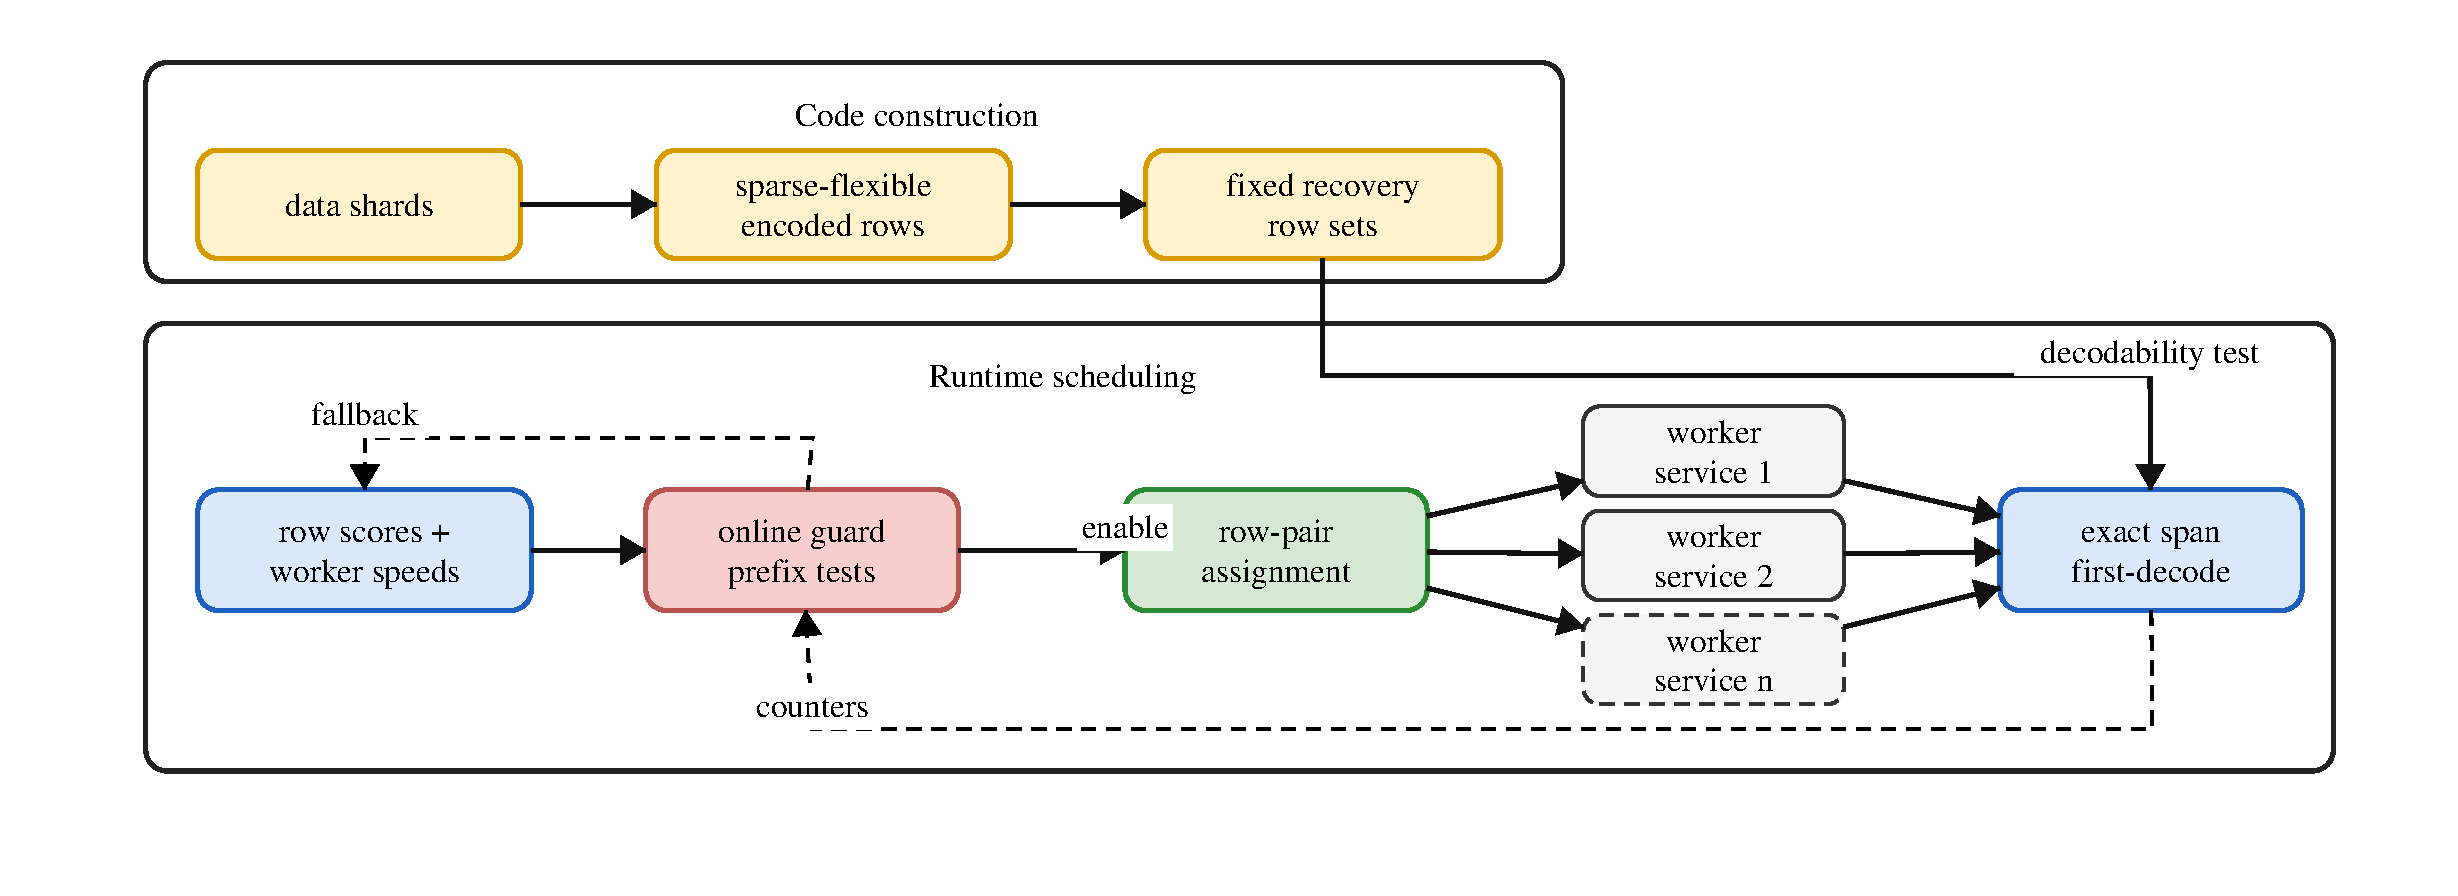
\includegraphics[width=\linewidth]{figures/figure1_architecture.pdf}
  \caption{Guarded first-decodable scheduling separates fixed code construction
  from runtime row exposure.}
  \Description{Two-lane architecture diagram. The top lane constructs fixed
  sparse-flexible encoded rows and recovery sets. The bottom lane uses row
  scores, worker speeds, an online guard, TCP worker services, and an exact
  first-decode monitor with counter feedback.}
  \label{fig:architecture}
\end{figure*}

\subsection{First-Decodable-Time Objective}

At iteration $t$, worker $j$ has a random completion time determined by its
current speed, queueing delay, and the sparse cost of the assigned row pair.
Let $\pi(i)$ denote the worker assigned to row pair $i$, containing rows $i$
and $i+n$ of the fixed code matrix $B$.  For a time $u$, let $S_\pi(u)$ be the
set of encoded rows completed by time $u$ under assignment $\pi$.

Under the exact row-span decoder used in this paper, the first decodable time is
\begin{equation}
  \label{eq:first-decodable-time}
  \tau(\pi, B) =
  \inf \{u : \mathbf{1}_m \in \mathrm{span}(B_{S_\pi(u)}^\top) \}.
\end{equation}
The system objective is
\begin{equation}
  \label{eq:first-decodable-objective}
  \min_\pi \mathbb{E}[\tau(\pi, B)].
\end{equation}

The objective in Equation~\eqref{eq:first-decodable-objective} differs from
minimizing total computation, assigned cost, or mean worker completion time.
It cares only about the earliest algebraically
sufficient set of returned rows.  The exact objective is combinatorial because
each completed subset has a different decodability status.  We therefore build
low-cost surrogates that preserve the central signal: how much a row
contributes to recovering the target vector $\mathbf{1}_m$.

\subsection{Target-Specific Decode Importance}

The scheduler needs a cheap signal for which encoded rows are useful for
recovering the target vector $\mathbf{1}_m$.  Let
$z\in\mathbb{R}^{2n}$ be a row-weight vector over all encoded rows of the fixed
code matrix $B$.  If every encoded gradient were available, coefficient $z_r$
would multiply the vector returned by row $r$.  The weighted sum recovers the
full gradient exactly when $B^\top z=\mathbf{1}_m$, because then the total
coefficient on every shard gradient is one.  Among all row-weight vectors that
satisfy this recovery condition, we choose the minimum-norm reference decoder
\begin{equation}
  \label{eq:reference-decoder}
  z^\star =
  \arg\min_z \|z\|_2^2
  \quad \mathrm{s.t.} \quad
  B^\top z = \mathbf{1}_m .
\end{equation}
When the target vector is recoverable from the full code matrix, this reference
decoder has the closed form
\begin{equation}
  \label{eq:reference-decoder-closed}
  z^\star = B(B^\top B)^\dagger \mathbf{1}_m .
\end{equation}
Equations~\eqref{eq:reference-decoder}
and~\eqref{eq:reference-decoder-closed} are computed only from the fixed code
matrix and the target full-gradient vector.  Here $(\cdot)^\dagger$ is the
Moore--Penrose pseudoinverse.  The vector
$z^\star$ is not the online decoder used after partial results arrive; online
decoding still solves the exact row-span condition on the returned subset.  We
use $z^\star$ only as a pre-runtime signal: if row $r$ has a large coefficient
in this reference decoder, delaying that row is more likely to delay a recovery
path for $\mathbf{1}_m$.  We therefore define the target-specific importance of
row $r$ as
\begin{equation}
  \label{eq:row-importance}
  \rho_r = |z^\star_r|.
\end{equation}

The runtime assigns row pairs rather than individual rows.  Pair $i$ contains
rows $i$ and $i+n$, and its sparse computation cost is $C_i$.  The scheduler
uses the pair priority
\begin{equation}
  \label{eq:pair-priority}
  R_i = (\rho_i + \rho_{i+n}) C_i,
\end{equation}
so a pair becomes high priority only when it is both decode-relevant and costly
enough for placement to matter.  Equation~\eqref{eq:pair-priority} is a
scheduling feature, not a
recovery certificate.  The runtime still accepts decoding only after the exact
row-span test succeeds on streamed completions.  Multiplying by $C_i$ is a
systems choice rather than a theorem: a high-$\rho$ row with negligible cost
does not need a scarce early worker, while a costly row matters only if it is
also decode-relevant.  The evaluation therefore treats score variants as
diagnostics, and the guard remains the protection against regimes where this
feature is misaligned with true first-decode criticality.

\subsection{Decode-Aware Assignment}

The decode-aware scheduler sorts row pairs by decreasing $R_i$ and workers by
decreasing estimated speed, then assigns the $k$th highest-priority row pair to
the $k$th fastest worker.  This simple monotone rule requires only the code
matrix and a current speed estimate.  It is
implemented as \textsc{RankAwareSparseFlexible} in the prototype.
The rule is deliberately conservative: it does not change the code, the number
of encoded rows, or the algebraic recovery condition.  It only permutes the
mapping between already-defined row pairs and available workers.

Algorithm~\ref{alg:decode-aware} shows the full scheduling path.  Lines 1--4
compute a target-specific decode-mass signal from the fixed code matrix.
Lines 5--7 lift that row-level signal to row pairs and multiply it by sparse
row-pair cost, because a high-importance row pair only changes wall-clock time
when its computation is nontrivial.  Lines 8--12 then perform the monotone
placement.  The important point is that $R_i$ is not treated as an independent
utility score for a completed row.  It is a proxy for how much delaying that
row pair can delay the first completed set whose span contains
$\mathbf{1}_m$.  Thus the scheduler tries to make the likely early prefix of
completed rows more decodable, rather than merely cheaper or faster in total.

\begin{algorithm}[t]
  \caption{Decode-aware row-pair assignment}
  \label{alg:decode-aware}
  \begin{algorithmic}[1]
    \Require Fixed code matrix $B$, pair costs $\{C_i\}$, worker speed estimates $\{s_j\}$
    \Ensure Row-pair to worker assignment $\pi$
    \State Compute $z^\star = B(B^\top B)^\dagger \mathbf{1}_m$
    \ForAll{encoded rows $r$}
      \State $\rho_r \gets |z^\star_r|$
    \EndFor
    \ForAll{row pairs $i$}
      \State $R_i \gets (\rho_i + \rho_{i+n}) C_i$
    \EndFor
    \State $(i_1,\ldots,i_n) \gets$ row pairs sorted by decreasing $R_i$
    \State $(j_1,\ldots,j_n) \gets$ workers sorted by decreasing $s_j$
    \For{$k=1,\ldots,n$}
      \State $\pi(i_k) \gets j_k$
    \EndFor
    \State \Return $\pi$
  \end{algorithmic}
\end{algorithm}

\subsection{Deadline-Aware Extension}

Decode-aware sorting is the main instantiation of the scheduling idea.  As a
stress-test extension for runtimes with transient delay, we also define a
deadline-aware matching score.  Let
\begin{equation}
  \label{eq:deadline-time}
  \widehat{T}_{ij} = d_j + \gamma C_i / s_j
\end{equation}
be the nominal completion time of pair $i$ on worker $j$, with delay $d_j$,
speed $s_j$, and runtime scale $\gamma$.  For a target deadline $q$, define the soft
completion probability
\begin{equation}
  \label{eq:deadline-probability}
  P_{ij}(q) = \exp(-\widehat{T}_{ij}/q).
\end{equation}
The scheduler solves
\begin{equation}
  \label{eq:deadline-assignment}
  \max_\pi \sum_i R_i P_{i,\pi(i)}(q),
\end{equation}
a standard linear assignment problem.  Equations~\eqref{eq:deadline-time},
\eqref{eq:deadline-probability}, and~\eqref{eq:deadline-assignment} define the
optional deadline-aware policy.  It builds
$W_{ij}=R_iP_{ij}(q)$ and calls \textsc{MaxWeightMatching}$(W)$, which returns
the assignment $\pi$ maximizing $\sum_i W_{i,\pi(i)}$.  In the current
prototype, $q$ is the median nominal completion time in the iteration.  The
extension is useful when transient delay makes the fastest worker by compute
speed differ from the earliest worker by response time.

\begin{algorithm}[t]
  \caption{Deadline-aware row-pair assignment}
  \label{alg:deadline-aware}
  \begin{algorithmic}[1]
    \Require Pair scores $\{R_i\}$, costs $\{C_i\}$, speeds $\{s_j\}$, delays $\{d_j\}$, deadline $q$
    \Ensure Row-pair to worker assignment $\pi$
    \ForAll{row pairs $i$ and workers $j$}
      \State $\widehat{T}_{ij} \gets d_j + \gamma C_i / s_j$
      \State $P_{ij}(q) \gets \exp(-\widehat{T}_{ij}/q)$
      \State $W_{ij} \gets R_i P_{ij}(q)$
    \EndFor
    \State $\pi \gets \Call{MaxWeightMatching}{W}$ \Comment{maximize $\sum_i W_{i,\pi(i)}$}
    \State \Return $\pi$
  \end{algorithmic}
\end{algorithm}

Algorithm~\ref{alg:decode-aware} requires one target-decoder computation when
the code changes and an $O(n\log n)$ sort per scheduling round.  The optional
deadline-aware variant adds an $n\times n$ weight matrix and a cubic-time exact
assignment solve.  It is therefore a stress-test policy, not the default path;
larger deployments can use the monotone sort, top-$k$ candidate matching, or
incremental rematching when few delay estimates change.

\subsection{Guard Enablement Conditions}

The scheduler is intentionally conditional: it is not expected to improve every
iteration.  It helps when two conditions hold.  First, static placement must be
misaligned with decode priority, so high-$R_i$ row pairs are not already on
workers likely to complete early.  Second, the reassignment must reduce the
arrival index of the first decodable set, or at least avoid increasing it by
more than the speedup can compensate.  In the prototype we expose this
through runtime counters for selected rows, completed rows, extra compute, and
scheduler time.  These counters are used in the evaluation to explain the
boundary between strong tail improvements and modest or negative gains.

This yields a fixed counter guard: enable adaptive assignment only when
estimated mismatch is positive and recent first-decode counters do not show a
larger completed-row prefix.  A payload $P=(B,\pi)$ combines the fixed code
matrix with a row-to-worker assignment.  \textsc{G-port}, the main system,
compares a safe fallback payload $P_0$ against candidate payloads and runs an
adaptive candidate only if every guard test passes.  Its
first-decode-aware coded
candidate is built by applying the row-pair scores from
Algorithm~\ref{alg:decode-aware} inside the deadline-aware matching of
Algorithm~\ref{alg:deadline-aware}; we call this coded candidate
\textsc{Guard-D}.  If the guard does not pass,
\textsc{G-port} falls back to static sparse-flexible placement.  Rank-only
ordering (\textsc{Guard-R}), coded-only \textsc{Guard-D}, and alternative
fallback choices are retained as ablations to isolate which part of the system
matters; they are not separate proposed methods.

Algorithm~\ref{alg:counter-guard} is the online guard used by the implemented
runtimes and replayed unchanged in diagnostic experiments.  In simulation and
replay studies, the rule is applied to recorded or synthesized worker states;
in multi-process and worker-service runs (TCP, Docker, and K3s), the master
executes it before each iteration.  The rule has four tests.  It first predicts
the static fallback
payload $P_0$ and the candidate coded payload $P_c$, then enables $P_c$ only
when worker speeds are heterogeneous enough, the predicted first-decode time is
lower, the predicted first-decode prefix does not grow, and recent monitored
counters do not show extra prefix growth or post-decode work.  Here
$\mathrm{cv}(\text{speed})$ is the coefficient of variation of the current
worker-speed estimates.  Thus the
decision is made before the iteration and cannot select a policy after seeing
that iteration's latency.

The counter update is conservative.  In cold start, the exponential
moving-average counters are zero, so the guard is controlled only by the current
worker state and the predicted static-vs-candidate prefix comparison.  After an
enabled round, the monitor updates the counters from the observed first-decode
event.  After a fallback round, the candidate did not run, so the counters decay
toward zero rather than being updated from the fallback's outcome.

\textsc{Predict} is an online model over current runtime features, not a replay
oracle.  For a payload $P=(B,\pi)$, it returns
$(\widehat{\tau},\widehat{K})$, where $\widehat{\tau}$ is predicted first-decode
time and $\widehat{K}$ is the predicted first-decodable prefix length.  Row $r$
assigned to worker $j=\pi(r)$ has nominal service time
\begin{equation}
  \label{eq:nominal-service}
  \widehat{x}_{rj}
  =
  \beta_d d_j + \beta_c c_r / \max(s_j,\epsilon),
\end{equation}
where $d_j$ and $s_j$ are the current delay and speed estimates, $c_r$ is row
cost, and $\beta_d,\beta_c$ are runtime scales.  If a worker receives multiple
rows, predicted completion is cumulative over its local queue:
\begin{equation}
  \label{eq:predicted-completion}
  \widehat{t}_r
  =
  \sum_{r' \preceq_j r} \max(0,\widehat{x}_{r'j}) .
\end{equation}
Here $r'\preceq_j r$ means row $r'$ is no later than $r$ in worker $j$'s queue.
Equations~\eqref{eq:nominal-service} and~\eqref{eq:predicted-completion}
therefore convert a payload into a predicted row-arrival order.
The predictor sorts rows by $\widehat{t}_r$ and runs the same incremental
row-span test as the decoder; the first successful arrival time is
$\widehat{\tau}$, and the successful prefix size is $\widehat{K}$.  Prediction
errors are handled conservatively by requiring positive predicted gain,
non-increasing predicted prefix, and non-growing EMA prefix counters before
enabling the candidate scheduler.

\begin{algorithm}[t]
  \caption{Online counter guard}
  \label{alg:counter-guard}
  \begin{algorithmic}[1]
    \Require Fallback payload $P_0$, candidate payload $P_c$, worker state,
      thresholds $\theta_{\mathrm{cv}},\theta_g,\theta_K,\theta_a$,
      EMA counters $\bar{\Delta K}$ and $\bar{A}$, update weight $\alpha_{\mathrm{ema}}$,
      fallback decay $\lambda$
    \Ensure Payload for this iteration and updated guard state
    \State Predict $(\hat{\tau}_0,\hat{K}_0)$ for $P_0$
    \State Predict $(\hat{\tau}_c,\hat{K}_c)$ for $P_c$
    \State $g \gets (\hat{\tau}_0-\hat{\tau}_c)/\hat{\tau}_0$
    \State $\Delta \hat{K}\gets \hat{K}_c-\hat{K}_0$
    \State $h\gets(\bar{\Delta K}\le\theta_K)\wedge(\bar{A}\le\theta_a)$
    \If{$\mathrm{cv}(\text{speed})\ge\theta_{\mathrm{cv}}$
        and $g\ge\theta_g$ and $\Delta\hat{K}\le\theta_K$ and $h$}
      \State run candidate scheduler $P_c$
      \State observe first-decodable prefix $K_c$ and rows-after-decode $A$
      \State $\bar{\Delta K}\gets(1-\alpha_{\mathrm{ema}})\bar{\Delta K}+\alpha_{\mathrm{ema}}(K_c-\hat{K}_0)$
      \State $\bar{A}\gets(1-\alpha_{\mathrm{ema}})\bar{A}+\alpha_{\mathrm{ema}} A$
    \Else
      \State run fallback $P_0$
      \State $\bar{\Delta K}\gets\lambda\bar{\Delta K}$; $\bar{A}\gets\lambda\bar{A}$
    \EndIf
  \end{algorithmic}
\end{algorithm}

\section{Surrogate Analysis}

\subsection{Recovery Preservation}

\textbf{Lemma 1.}
For a fixed sparse flexible code $B$, any row assignment or row permutation
preserves the algebraic recovery capability of the code.

\textit{Proof sketch.}
Assignment changes when rows arrive, not the row space generated by all rows.
For any permutation matrix $P$, $\mathrm{rank}(B)=\mathrm{rank}(PB)$ and
$\mathbf{1}_m \in \mathrm{span}(B^\top)$ if and only if
$\mathbf{1}_m \in \mathrm{span}((PB)^\top)$.  Therefore scheduling can improve
the first decodable time without weakening the underlying recovery threshold.

\subsection{Decode-Mass Surrogate}

Fix a deadline $u$.  Suppose worker $j$ completes its assigned row pair before
$u$ with probability $p_j(u)$, and $p_j(u)$ is monotone in worker speed.  A
natural surrogate for early decodability is expected completed decode mass:
\begin{equation}
  \label{eq:decode-mass-surrogate}
  \max_\pi \sum_i p_{\pi(i)}(u) R_i .
\end{equation}

\textbf{Lemma 2.}
The optimal assignment for the surrogate in
Equation~\eqref{eq:decode-mass-surrogate} pairs the largest $R_i$ with the
largest $p_j(u)$, the second largest with the second largest, and so on.

\textit{Proof sketch.}
The result follows from the rearrangement inequality.  For any inversion where
$R_a \ge R_b$ but $p_{\pi(a)} < p_{\pi(b)}$, swapping the two assignments
changes the objective by
$(R_a-R_b)(p_{\pi(b)}-p_{\pi(a)}) \ge 0$.  Repeatedly removing inversions gives
the monotone assignment.

\subsection{Mismatch Creates Scheduling Opportunity}

The preceding surrogate also gives a way to state when decode-aware scheduling
has room to help.  Let $q_j(u)=p_j(u)$ be the probability that worker $j$
finishes before deadline $u$, and let $\pi_0$ be the static row-pair placement.
Define the normalized decode-speed mismatch
\begin{equation}
  \label{eq:mismatch-score}
  M(\pi_0,u)
  =
  \frac{
    \max_\pi \sum_i R_i q_{\pi(i)}(u)
    -
    \sum_i R_i q_{\pi_0(i)}(u)
  }{
    \max_\pi \sum_i R_i q_{\pi(i)}(u)
    -
    \min_\pi \sum_i R_i q_{\pi(i)}(u)
  } . 
\end{equation}
In Equation~\eqref{eq:mismatch-score}, the numerator is the decode-mass
headroom left by the static placement
$\pi_0$: it compares the best assignment at deadline $u$ with the assignment
the fixed runtime would have used.  The denominator is the full feasible range
between the best and worst assignments, so the ratio normalizes the score to
$[0,1]$ when worker probabilities and row priorities are not both constant.
$M=0$ means the static placement is already optimal for this surrogate; $M=1$
means it is maximally anti-aligned.  The score is an opportunity signal, not a
latency guarantee.

\textbf{Lemma 3.}
If $M(\pi_0,u)=0$, no reassignment can improve the expected decode-mass
surrogate at deadline $u$.  If $M(\pi_0,u)>0$, the best monotone reassignment
improves the surrogate by exactly $M(\pi_0,u)$ times the surrogate's assignment
range.

\textit{Proof sketch.}
The definition subtracts the static surrogate value from the optimal surrogate
value and normalizes by the feasible range.  Lemma 2 identifies the optimizer
as the monotone assignment.  Therefore zero mismatch means there is no
decode-mass opportunity, while positive mismatch quantifies the available
surrogate improvement.

\subsection{Prefix Reduction Realizes Latency Gain}

The mismatch score says that reassignment has room to help, but it does not by
itself imply lower latency.  The benefit appears only when a decodable row set
arrives earlier.  For an assignment $\pi$, order returned rows by arrival time
and let $T_{\pi,(k)}$ be the time of the $k$th arrival.  Define
\begin{equation}
  \label{eq:first-decodable-prefix}
  K_\pi = \min\{k : \text{the first } k \text{ arrivals under } \pi
  \text{ are decodable}\}.
\end{equation}
Equation~\eqref{eq:first-decodable-prefix} defines the first-decodable prefix
length: the number of completed rows needed before the row-span decoder can
recover the full gradient.  If $h_\pi$ is scheduling and monitoring overhead,
the first-decode time is
\begin{equation}
  \label{eq:first-decode-overhead}
  \tau_\pi = T_{\pi,(K_\pi)} + h_\pi .
\end{equation}

This gives the guard's decision criterion.  Compare static placement $\pi_0$
with adaptive placement $\pi$.  If the candidate does not increase the required
prefix ($K_\pi\le K_{\pi_0}$), the predicted gain can be written as
\begin{equation}
  \label{eq:prefix-gain-decomposition}
  \tau_{\pi_0}-\tau_\pi
  =
  \underbrace{T_{\pi_0,(K_{\pi_0})}-T_{\pi_0,(K_\pi)}}_{\text{fewer rows waited for}}
  +
  \underbrace{T_{\pi_0,(K_\pi)}-T_{\pi,(K_\pi)}}_{\text{same prefix arrives earlier}}
  -
  h_\pi .
\end{equation}
Equation~\eqref{eq:prefix-gain-decomposition} separates three effects: prefix
reduction, faster placement for the same prefix length, and overhead.  This is
why the guard rejects candidates that predict a longer prefix or too much
post-decode work: speed alone is insufficient unless the candidate exposes a
decodable prefix early enough to pay for scheduling, communication, and
cancellation overhead.

\subsection{Surrogate Rationale and Limits}

The exact event of interest is whether the rows completed by deadline $u$ form a
decodable set.  If $\mathcal{D}$ is the family of row subsets that can decode
the target vector, then
\begin{equation}
  \label{eq:decodable-event}
  \Pr[\tau(\pi,B) \le u]
  =
  \Pr[S_\pi(u) \in \mathcal{D}].
\end{equation}
Computing Equation~\eqref{eq:decodable-event} exactly requires reasoning over
many completed
subsets.  The decode-mass surrogate uses a scalar proxy instead: let
$Z_{\pi,i}(u)$ indicate whether row pair $i$ finishes before $u$, and define
$X_\pi(u)=\sum_i R_i Z_{\pi,i}(u)$.  A threshold relaxation treats a row set as
promising when $X_\pi(u)\ge\theta$.  Increasing
$\mathbb{E}[X_\pi(u)]$ therefore improves this relaxed event when variance does
not grow enough to offset the mean gain.

This is a runtime proxy, not a correctness argument.  A large $R_i$ suggests
that row pair $i$ is useful to expose early, but it does not certify that any
returned subset is decodable.  The runtime uses the surrogate only to choose an
assignment; correctness still comes from the exact online row-span decoder.  The
guard rejects the surrogate when predicted prefix or overhead counters indicate
that the proxy is unreliable.

\section{Experimental Setup}
\label{sec:setup}
\label{sec:experimental-setup}

\subsection{Workloads and Worker Traces}

We use a controlled sparse ridge-regression workload for the main experiments.
The generator creates a sparse feature matrix, partitions it into shards, and
computes one additive gradient contribution per shard.  A successful coded
decode therefore recovers the same full gradient as the uncoded shard sum, which
matches the linear aggregation model used by gradient coding~\cite{tandon2017gradient}
and sparse flexible coded learning~\cite{zhang2025sparseflexible}.  We use this
workload to isolate row-span recoverability, sparse row cost, and first-decode
timing, not to claim a full training-stack speedup for all sparse models.

Worker-state streams are controlled stress traces generated by the runtime.
Each iteration supplies per-worker speeds, straggler delays, and a slow-worker
mask.  We use four regimes: stable lognormal heterogeneity, bursty stragglers,
drifting base speeds, and phase changes in straggler fraction and slowdown.
These regimes model late-task effects in cluster systems~\cite{zaharia2008late}
and heterogeneous ML scheduling effects~\cite{narayanan2020gavel}.  The main
SoCC-facing experiments use phase-changing streams because the relative
importance of speed, delay, and row cost changes over time.  The traces are
controlled rather than production logs, so every paired comparison reuses the
same worker-state stream across strategies within a run.

\subsection{Metrics and Accounting}

Recent cluster schedulers report completion time, waiting time or slowdown,
resource utilization, and scheduling overhead~\cite{dongare2025rltune};
distributed-training planners additionally report throughput, cost, and search
time~\cite{strati2025sailor}.  Our setting has one synchronous coded-learning
iteration rather than a queue of multi-job training requests, so we adapt these
metrics to worker-service rounds.  The names below are the names used in the
evaluation tables and figures.
\begin{enumerate}
\setlength{\itemsep}{2pt}
\item \textbf{Mean barrier latency (\emph{Mean (ms)} or \emph{Barrier (ms)}).}
This is the end-to-end synchronous iteration time.  It includes first decode,
stream cancellation, and worker cleanup, which makes it the main metric for
deployed worker-service runs.  Stress tables use \emph{Barrier (ms)} for the
same quantity.
\item \textbf{Tail latency (\emph{p95 (ms)}).}  Tail latency is a standard
systems metric for cloud services~\cite{dean2013tail}.  We report p95 because
first-decode savings are useful only if they survive tail workers,
cancellation, and communication cleanup.
\item \textbf{Throughput (\emph{Thr. (iter/s)}).}  Training planners and cluster schedulers
commonly report throughput or goodput~\cite{strati2025sailor,qiao2021pollux}.
We use the reciprocal of barrier latency, reported as completed coded-learning
iterations per second.
\item \textbf{Worker-service overhead (\emph{Post rows} and \emph{Cancel (ms)}).}
Recent schedulers report scheduling runtime, search time, or planner overhead
alongside end-to-end performance~\cite{dongare2025rltune,strati2025sailor}.  In
our tables, \emph{Post rows} is the number of row results completed after the
first decodable event but before the round finishes, and \emph{Cancel (ms)} is
the cancellation/cleanup time included in the barrier path.  Lower values mean
less wasted work or less cleanup delay.
\item \textbf{Correctness and recovery counters (\emph{Succ.}, \emph{Gain},
\emph{Err.}, and \emph{Recov.}).}  Coded learning requires recovering the
intended gradient or row span despite
stragglers~\cite{tandon2017gradient,zhang2025sparseflexible}, while distributed
training systems also track worker faults and failure reactions~\cite{deng2025minder}.
\emph{Succ.} is the decode-success rate.  \emph{Gain} is the percentage
improvement over the comparison reference stated by the table or figure, such
as SFCL in the stress table.  \emph{Err.} is closed-worker errors per round, and
\emph{Recov.} is bounded row reissues per round.
\item \textbf{Mechanism and guard diagnostics.}  The row-exposure diagnostic
reports \emph{Mean gain}, \emph{p95 gain}, and $\Delta$ \emph{prefix}, all
relative to static placement in the same diagnostic.  Guard figures and tables
report \emph{decision rate}, \emph{false-enable rate}, \emph{false-disable
rate}, \emph{Mean/p95 $\tau$ error}, and \emph{Prefix-length error}.  Decision
rate is the fraction of rounds in which the guard enables adaptive scheduling;
false-enable and false-disable rates come from paired replay on the same
worker-state stream.
\end{enumerate}

These metrics test whether first-decode prefix savings survive scheduling,
communication, and cleanup costs.  Operationally, the scheduler should be
enabled only when the expected prefix saving exceeds the overhead budget,
\[
  \Delta T_{\mathrm{prefix}} >
  T_{\mathrm{sched}} + T_{\mathrm{extra}} + T_{\mathrm{cancel/comm}} .
\]

Replication counts, run identifiers, and raw per-run latency traces are
artifact details.  The main text keeps aggregate barrier, tail, throughput,
overhead, decision, and recovery results; the artifact retains the complete run
matrix, arm selections, paired comparisons, resource counters, and scripts that
regenerate the tables.

\subsection{Baselines and External Adapters}

The main comparison uses same-runtime baselines so that every method shares the
same sparse workload, worker-state stream, serialization path, cancellation
logic, and barrier accounting.  We use the following comparison points.
\begin{enumerate}
\setlength{\itemsep}{2pt}
\item \textbf{SFCL.}  This is the closest coded-computing baseline: static
sparse-flexible coded placement from SFCL~\cite{zhang2025sparseflexible}.  We
reimplement it in the same runtime.  It fixes the encoded-row assignment before
each round and uses neither worker heterogeneity nor first-decode prefix
features.
\item \textbf{RLTune-style adapter.}  This adapter follows the systems role of
RLTune~\cite{dongare2025rltune} by selecting among uncoded, speculative,
static-coded, and rank-aware coded arms using runtime heterogeneity features.
It is a same-runtime adapter, not a port of the full RLTune scheduler.
\item \textbf{Sailor-style adapter.}  This adapter follows the speed/cost
modeling role of Sailor~\cite{strati2025sailor}.  It assigns work using
worker-speed and row-cost estimates, but it does not use coded row-span or
first-decodable-prefix features.
\end{enumerate}

\textbf{Guarded enablement.}
The guard used in the evaluation is a deployment rule over runtime counters,
not a selector trained on final latency.  The online runtime estimates
decode-speed mismatch from row priorities and worker-speed estimates before an
iteration starts, predicts if the adaptive policy will shorten the
first-decodable prefix, and updates counters after the observed first-decode
event.  If the predicted prefix is worse, or recent counters show that adaptive
assignment expanded the completed-row prefix, \textsc{G-port} rejects the
adaptive arm and falls back to static sparse-flexible placement.  The portfolio
candidates share the same worker-service accounting; the ablations then remove
cross-policy execution or change the fallback rule.  The \texttt{best\_safe}
ablation chooses the cheaper predicted safe baseline between speed-aware
uncoded and static coded placement before the round.  Paired safe-baseline
replays over logged diagnostics estimate fallback headroom; they do not relabel
deployed K3s traces.  Unless stated otherwise,
the guard thresholds are $\theta_{\mathrm{cv}}=0.20$, $\theta_g=0.01$,
$\theta_K=0$ rows, and $\theta_a=1$ row; the EMA update weight is
$\alpha_{\mathrm{ema}}=0.30$ and the fallback decay is $\lambda=0.80$.

\subsection{Runtime Prototypes}

The experiments use three Python runtimes for sparse coded learning.  The
labels in Table~\ref{tab:external-main} are configurations of the
worker-service runtime: TCP runs local worker services over sockets,
TCP+stress adds analytic request/response delay and bandwidth limits to the
same TCP path, and K3s runs the same worker entrypoint as pods behind headless
Services.  The simulator and multi-process runtimes support mechanism checks;
the main external comparison uses the TCP-family and K3s worker-service
realizations.
\begin{enumerate}
\setlength{\itemsep}{2pt}
\item \textbf{Event simulator.}\par
The simulator generates sparse ridge data,
partitions it into shards, constructs the fixed sparse-flexible code matrix, and
samples worker completion times from the configured trace.  It runs the exact
row-span decoder after each row arrival.  We use it for mechanism sweeps,
oracle diagnostics, threshold sensitivity, and paired replays because it
separates scheduling logic from process, socket, and container overheads.

\item \textbf{Multi-process runtime.}\par
The local runtime starts one Python
worker process per logical worker.  The master assigns encoded row pairs,
workers compute sparse encoded gradients over their assigned shard
combinations, and completed rows are streamed back to the master.  After the
first decodable set is reached, the master cancels remaining work and records
both first-decode latency and conservative barrier latency, including
cancellation cleanup.  This runtime validates the master/worker control path
without network isolation.

\item \textbf{TCP worker-service runtime.}\par
The worker-service runtime launches
each worker as an independent TCP service.  Master and workers exchange
length-prefixed task, row, cancel, stop, and acknowledgement messages.  A task
message carries the round id, row ids, encoded rows, worker speed/delay state,
and current model vector; row messages return encoded gradients, row cost,
payload size, and timing counters.  The same worker entrypoint runs as local
services, host-published Docker containers, Docker-bridge containers, and
three-node K3s pods reached through headless Services.  This validates the
worker-service boundary without publishing worker ports.  For restricted cloud
hosts, the runtime also supports an SSH-forwarded two-node mode.  The K3s run is
a shared-pod validation, not an isolated production cluster; pod placement,
resource knobs, and manifests are artifact metadata.  The runtime also includes
the closed-connection stress hook: if a worker disconnects before first decode,
the master marks it unavailable, filters unfinished rows that have not arrived,
and reissues them to the fastest live worker.  Exact decoding remains the
correctness test; if reissued rows do not arrive in time, the iteration fails
normally and the next round can fall back to SFCL.
\end{enumerate}

The current runtimes are still prototypes: they de-risk the service boundary,
cancellation path, and small pod-to-pod TCP deployment, while production-scale
cluster scheduling and interference remain future systems work.  This is a
deployment step rather than a different algorithmic path, because the scheduler
only depends on streamed completions and cancellation acknowledgments.

\section{Evaluation}
\label{sec:evaluation}

We evaluate \textsc{G-port} as a runtime scheduling layer, not a new code
construction.  The evaluation first compares \textsc{G-port} with same-runtime
external adapters across TCP, stressed TCP, and K3s worker services, then
isolates design choices, guard sensitivity, stress recovery, and row-exposure
mechanisms.  The main comparison reports latency, tail latency, throughput, work
overhead, cancellation cost, and decode success; later diagnostics reuse the
decision and recovery counters from Section~\ref{sec:setup}.

\subsection{Main External Comparison}

Table~\ref{tab:external-main} is the main systems result.  Every row uses the
same payloads, worker-state streams, cancellation path, and barrier accounting
inside that runtime.  RLTune and Sailor are same-runtime scheduler adapters, not
full system ports; they test whether generic heterogeneity-aware scheduling is
enough once the runtime and workload are held fixed.  The table reports raw
metrics rather than normalized gains: mean barrier latency, p95 barrier latency,
achieved iteration throughput, post-decode rows, cancellation time, and decode
success.

\begin{table*}[t]
  \centering
  \caption{Main external comparison.}
  \label{tab:external-main}
  \begin{tabular*}{\textwidth}{@{\extracolsep{\fill}}lllrrrrrr@{}}
    \toprule
    Runtime & Workers & Method & Mean & p95 & Thr. & Post & Cancel & Succ. \\
            &         &        & (ms) & (ms) & (iter/s) & rows & (ms) & \\
    \midrule
    TCP & W8 & SFCL & 44.0 & 80.5 & 22.7 & 1.8 & 16.8 & 1.00 \\
        &    & RLTune & 48.2 & 76.6 & 20.8 & 0.1 & 16.5 & 1.00 \\
        &    & Sailor & 53.9 & 77.8 & 18.6 & 0.0 & 19.2 & 1.00 \\
        &    & \textsc{G-port} & \textbf{40.9} & \textbf{71.5} & \textbf{24.4} & 1.6 & 14.1 & 1.00 \\
        & W16 & SFCL & 38.3 & \textbf{48.3} & 26.1 & 10.4 & 16.5 & 1.00 \\
        &     & RLTune & 36.4 & 59.1 & 27.4 & 1.4 & 16.5 & 1.00 \\
        &     & Sailor & \textbf{35.3} & 59.5 & \textbf{28.3} & 0.0 & 16.3 & 1.00 \\
        &     & \textsc{G-port} & 36.6 & 60.0 & 27.4 & 4.1 & 16.9 & 1.00 \\
        & W24 & SFCL & 47.5 & 62.3 & 21.1 & 21.9 & 21.4 & 1.00 \\
        &     & RLTune & 48.3 & \textbf{59.9} & 20.7 & 2.8 & 24.2 & 1.00 \\
        &     & Sailor & 44.3 & 61.1 & 22.6 & 0.0 & 21.8 & 1.00 \\
        &     & \textsc{G-port} & \textbf{43.7} & 61.1 & \textbf{22.9} & 1.7 & 20.5 & 1.00 \\
    \midrule
    TCP+stress & W8 & SFCL & 49.4 & 88.6 & 20.2 & 1.4 & 15.2 & 1.00 \\
        &    & RLTune & 55.6 & 86.0 & 18.0 & 0.3 & 17.1 & 1.00 \\
        &    & Sailor & 56.3 & 89.9 & 17.8 & 0.0 & 15.8 & 1.00 \\
        &    & \textsc{G-port} & \textbf{48.4} & \textbf{73.9} & \textbf{20.7} & 1.6 & 15.2 & 1.00 \\
        & W16 & SFCL & 53.2 & \textbf{71.0} & 18.8 & 9.8 & 23.6 & 1.00 \\
        &     & RLTune & 53.1 & 77.0 & 18.8 & 1.5 & 22.5 & 1.00 \\
        &     & Sailor & 53.3 & 71.2 & 18.7 & 0.0 & 22.2 & 1.00 \\
        &     & \textsc{G-port} & \textbf{53.1} & 83.9 & \textbf{18.8} & 0.0 & 22.2 & 1.00 \\
        & W24 & SFCL & 60.9 & 93.3 & 16.4 & 21.0 & 27.2 & 1.00 \\
        &     & RLTune & 65.4 & 137.5 & 15.3 & 4.1 & 29.8 & 1.00 \\
        &     & Sailor & 55.5 & 67.6 & 18.0 & 0.0 & 23.9 & 1.00 \\
        &     & \textsc{G-port} & \textbf{53.9} & \textbf{61.2} & \textbf{18.5} & 0.0 & 23.7 & 1.00 \\
    \midrule
    K3s & W8 & SFCL & 22.7 & 60.3 & 44.0 & 0.4 & 1.7 & 1.00 \\
        &    & RLTune & 28.0 & 55.5 & 35.7 & 0.0 & 1.6 & 1.00 \\
        &    & Sailor & 29.0 & 54.4 & 34.5 & 0.0 & 1.6 & 1.00 \\
        &    & \textsc{G-port} & \textbf{19.6} & \textbf{42.0} & \textbf{51.0} & 0.4 & 1.7 & 1.00 \\
        & W16 & SFCL & 14.5 & 16.3 & 69.1 & 3.4 & 3.6 & 1.00 \\
        &     & RLTune & 9.8 & 10.9 & 102.0 & 1.3 & 3.2 & 1.00 \\
        &     & Sailor & \textbf{9.4} & \textbf{10.2} & \textbf{106.7} & 0.0 & 2.9 & 1.00 \\
        &     & \textsc{G-port} & 11.3 & 16.0 & 88.3 & 1.5 & 3.2 & 1.00 \\
        & W24 & SFCL & 15.7 & 17.6 & 63.6 & 8.9 & 5.6 & 1.00 \\
        &     & RLTune & 12.8 & 14.8 & 78.2 & 2.5 & 4.6 & 1.00 \\
        &     & Sailor & \textbf{12.4} & 13.3 & \textbf{80.8} & 0.0 & 4.3 & 1.00 \\
        &     & \textsc{G-port} & 12.4 & \textbf{13.2} & 80.5 & 0.0 & 4.3 & 1.00 \\
    \bottomrule
  \end{tabular*}
\end{table*}

The table makes the runtime boundary explicit: the same adapter set runs under
local TCP, stressed TCP, and pod-to-pod K3s services.  Generic heterogeneity
schedulers improve selected W16/W24 cases but regress at W8 because they do not
control which coded rows make the first decodable prefix appear.  \textsc{G-port}
is not always fastest (Sailor wins some K3s W16/W24 speed-dominated cases), but
it has the best W8 mean/p95 in all three runtimes, the best stressed-TCP W24
mean/p95, and competitive K3s W24 throughput.  The integrated overhead rows show
that the gain is not only a latency artifact: \textsc{G-port} usually leaves
fewer post-decode rows than SFCL and preserves decode success while cancellation
time remains included in the barrier path.  The artifact keeps completed rows,
extra work, dispatch time, bytes, per-seed traces, paired gains, and paired CIs.

\subsection{Ablation Study}

Table~\ref{tab:gport-ablation} removes deployable pieces of \textsc{G-port} in
all three runtimes.  \emph{w/o FD} removes first-decode-aware row ordering and
therefore becomes the Sailor-style speed/cost scheduler.  \emph{w/o code}
removes the code-aware candidate and becomes the RLTune-style heterogeneity
selector.  \emph{w/o portfolio} disables the cross-policy wrapper and runs the
coded-only \textsc{Guard-D} arm.  Each cell is mean latency / post-decode rows /
cancellation time; lower is better.

\begin{table*}[t]
  \centering
  \caption{\textsc{G-port} ablations.}
  \label{tab:gport-ablation}
  \begin{tabular*}{\textwidth}{@{\extracolsep{\fill}}llccc@{}}
    \toprule
    Runtime & Ablation & W8 & W16 & W24 \\
    \midrule
    \multicolumn{5}{@{}l@{}}{\emph{Cell:} mean ms / post rows / cancel ms} \\
    \midrule
    TCP & \textsc{G-port} & 40.9/1.6/14.1 & 36.6/4.1/16.9 & 43.7/1.7/20.5 \\
        & w/o FD          & 53.9/0.0/19.2 & 35.3/0.0/16.3 & 44.3/0.0/21.8 \\
        & w/o code        & 48.2/0.1/16.5 & 36.4/1.4/16.5 & 48.3/2.8/24.2 \\
        & w/o portfolio   & 43.3/1.6/17.6 & 38.5/10.6/15.4 & 47.0/22.1/21.0 \\
    \midrule
    TCP+stress & \textsc{G-port} & 48.4/1.6/15.2 & 53.1/0.0/22.2 & 53.9/0.0/23.7 \\
        & w/o FD          & 56.3/0.0/15.8 & 53.3/0.0/22.2 & 55.5/0.0/23.9 \\
        & w/o code        & 55.6/0.3/17.1 & 53.1/1.5/22.5 & 65.4/4.1/29.8 \\
        & w/o portfolio   & 47.9/2.0/15.3 & 55.8/11.1/24.8 & 54.7/19.7/24.6 \\
    \midrule
    K3s & \textsc{G-port} & 19.6/0.4/1.7 & 11.3/1.5/3.2 & 12.4/0.0/4.3 \\
        & w/o FD          & 29.0/0.0/1.6 & 9.4/0.0/2.9 & 12.4/0.0/4.3 \\
        & w/o code        & 28.0/0.0/1.6 & 9.8/1.3/3.2 & 12.8/2.5/4.6 \\
        & w/o portfolio   & 20.3/0.5/1.7 & 14.2/3.6/3.6 & 15.9/9.1/5.7 \\
    \bottomrule
  \end{tabular*}
\end{table*}

The ablation shows why the full controller is useful.  Speed/cost scheduling is
strong when speed dominates (K3s W16/W24) but fragile at W8 and under TCP stress.
The heterogeneity selector helps selected counts but has the largest stressed-TCP
W24 latency.  The w/o-portfolio variant is a clean coded-only ablation and
competitive at W8, but it loses the cross-policy fallback that protects
\textsc{G-port} when uncoded or speed-aware execution is temporarily safer.

\subsection{Guard Sensitivity}

\begin{figure}[t]
  \centering
  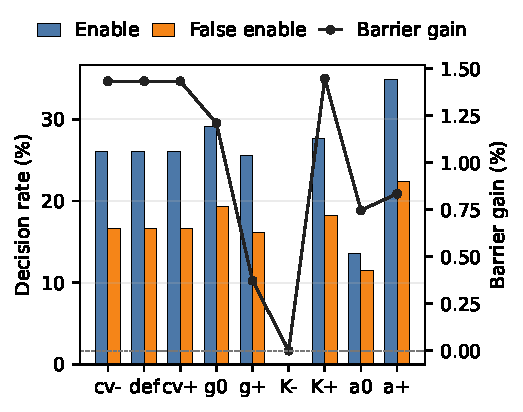
\includegraphics[width=\columnwidth]{figures/guard_threshold_sensitivity.pdf}
  \caption{Guard-threshold sensitivity.}
  \Description{Bar and line chart showing enable rate, false-enable rate, and
  barrier gain under small guard-threshold changes.}
  \label{fig:guard-thresholds}
\end{figure}

\begin{table}[t]
  \centering
  \caption{Figure~\ref{fig:guard-thresholds} settings.}
  \label{tab:guard-threshold-settings}
  \begin{tabular}{@{}lrrrr@{}}
    \toprule
    Label & theta-cv & theta-g & theta-K & theta-a \\
    \midrule
    low theta-cv & 0.10 & 0.01 & 0 & 1 \\
    default & 0.20 & 0.01 & 0 & 1 \\
    high theta-cv & 0.35 & 0.01 & 0 & 1 \\
    zero theta-g & 0.20 & 0.00 & 0 & 1 \\
    high theta-g & 0.20 & 0.03 & 0 & 1 \\
    strict theta-K & 0.20 & 0.01 & -1 & 1 \\
    loose theta-K & 0.20 & 0.01 & 1 & 1 \\
    strict theta-a & 0.20 & 0.01 & 0 & 0 \\
    loose theta-a & 0.20 & 0.01 & 0 & 2 \\
    \bottomrule
  \end{tabular}
\end{table}

Figure~\ref{fig:guard-thresholds} replays small threshold changes on paired K3s
guard rounds, and Table~\ref{tab:guard-threshold-settings} maps each x-axis
label to the guard rule.  Each non-default setting changes one gate while
holding the other three at the deployed default.  Here
theta-cv gates worker-speed heterogeneity, theta-g gates
predicted first-decode gain, theta-K gates the candidate-minus-fallback
first-decodable prefix delta, and theta-a gates rows of work completed after
decode.  Lower theta-K or theta-a values are stricter because they allow
less prefix growth or post-decode work.  Bars report enable decision rate and
false-enable rate; the line shows barrier gain.  Stricter thresholds reduce
false enables but also leave useful opportunities unused, so the default is a
conservative middle point rather than a tuned post-hoc optimum.

\subsection{Stress and Recovery}

Table~\ref{tab:k8s-stress} reports K3s W24 stress tests using the correctness
and recovery counters from Section~\ref{sec:setup}.  \emph{Stress} is the
injected runtime condition, not a new workload: Base has no injection, Cancel+20
delays cancellation, CPU hog adds co-located interference, Close closes one
worker connection, and Close+R repeats Close with bounded reissue.  Succ. is
decode success; Gain is relative to SFCL in the same stress; Err. and Recov. are
closed-worker errors and bounded reissues per round.

\begin{table}[t]
  \centering
  \setlength{\tabcolsep}{1.0pt}
  \caption{K3s W24 recovery counters.}
  \label{tab:k8s-stress}
  \begin{tabular}{@{}llrrrrrr@{}}
    \toprule
    Stress & Method & Succ. & Barrier & Gain & Err. & Recov. & Cancel \\
         &        &       & (ms) &      & /round & /round & (ms) \\
    \midrule
    Base & SFCL & 1.00 & 16.6 & 0.0\% & 0.00 & 0.00 & 5.7 \\
    Base & \textsc{G-port} & 1.00 & 12.6 & 23.7\% & 0.00 & 0.00 & 4.4 \\
    Base & Guard-D & 1.00 & 16.6 & -0.3\% & 0.00 & 0.00 & 5.6 \\
    \midrule
    Cancel+20 & SFCL & 1.00 & 33.7 & 0.0\% & 0.00 & 0.00 & 24.8 \\
    Cancel+20 & \textsc{G-port} & 1.00 & 32.0 & 5.1\% & 0.00 & 0.00 & 23.6 \\
    Cancel+20 & Guard-D & 1.00 & 33.9 & -0.7\% & 0.00 & 0.00 & 24.7 \\
    \midrule
    CPU hog & SFCL & 1.00 & 16.6 & 0.0\% & 0.00 & 0.00 & 5.6 \\
    CPU hog & \textsc{G-port} & 1.00 & 12.5 & 24.8\% & 0.00 & 0.00 & 4.3 \\
    CPU hog & Guard-D & 1.00 & 16.5 & 0.6\% & 0.00 & 0.00 & 5.5 \\
    \midrule
    Close & SFCL & 1.00 & 16.7 & 0.0\% & 1.00 & 0.00 & 5.5 \\
    Close & \textsc{G-port} & 0.67 & 10.8 & 35.0\% & 1.00 & 0.00 & 2.8 \\
    Close & Guard-D & 1.00 & 16.6 & 0.1\% & 1.00 & 0.00 & 5.5 \\
    \midrule
    Close+R & SFCL & 1.00 & 16.8 & 0.0\% & 1.00 & 1.00 & 5.7 \\
    Close+R & \textsc{G-port} & 1.00 & 12.7 & 24.2\% & 1.00 & 0.33 & 4.4 \\
    Close+R & Guard-D & 1.00 & 16.8 & 0.2\% & 1.00 & 1.00 & 5.7 \\
    \bottomrule
  \end{tabular}
\end{table}

The cases separate cleanup, interference, and connection-loss effects.  CPU hog
keeps the gain, while delayed cancellation shrinks it to 5.1\%.  Close without
recovery is only a diagnostic failure mode: fast successful rounds but 67\%
decode success.  Bounded reissue restores success to 1.0 and keeps a 24.2\%
gain, so we claim single-connection recovery semantics rather than production
fault tolerance.

\subsection{Mechanism: Row Exposure}

Table~\ref{tab:score-diagnostic} is an offline 8-worker/8-shard replay, not a
TCP or K3s deployment.  It fixes the code and worker states, changes only
row-pair priority, and measures predicted first-decode time.  The oracle is not
deployable; it only shows the headroom from exposing decode-important rows
earlier.  The cheap runtime score helps p95 but not mean latency, so
\textsc{G-port} treats row score as a guarded runtime feature.

\begin{table}[t]
  \centering
  \setlength{\tabcolsep}{1.0pt}
  \caption{Offline row-exposure replay.}
  \label{tab:score-diagnostic}
  \begin{tabular}{@{}lrrrrr@{}}
    \toprule
    Priority & FD mean & FD p95 & Mean gain & p95 gain & $\Delta$ prefix \\
             & (ms) & (ms) & & & \\
    \midrule
    Static & 31.6 & 117.0 & 0.0\% & 0.0\% & 0.0 \\
    Cost-only & 25.4 & 60.8 & 19.5\% & 48.1\% & -0.4 \\
    Runtime score & 32.8 & 85.6 & -3.8\% & 26.8\% & 0.0 \\
    Oracle-minset & 19.3 & 52.6 & 38.9\% & 55.1\% & -1.2 \\
    Random & 38.2 & 141.2 & -21.1\% & -20.7\% & +0.5 \\
    \bottomrule
  \end{tabular}
\end{table}

Full row-score sweeps, sampled-minset variants, score-build times, and per-seed
ranges are artifact material.  Among the five priorities, \textsc{G-port} uses
the deployable \emph{Runtime score} priority inside its Guard-D coded arm; Static,
Cost-only, Oracle-minset, and Random are controls that respectively represent
the SFCL baseline, a cost-only scheduler, a nondeployable upper-bound oracle, and
a sanity lower bound.  This diagnostic supports a narrow claim: decodability
features create useful candidates, and the online guard decides when to trust the
runtime score.

\subsection{Limitations}

This is a prototype validation: multi-process runs measure sparse kernels; TCP
adds serialization and cancellation; network stress adds analytic RTT/bandwidth;
Docker and K3s validate containerized worker-service paths at local and small
multi-node scales.  The K3s pods do not reserve exclusive CPU or memory.  The
artifact keeps pod placement, events, resource-counter snapshots when available,
and Docker stress hooks for slow cancellation, closed TCP connections, and
worker exits.  The prototype handles one closed connection by bounded row
reissue, but production scheduling, interference control, replicated master
state, multi-failure recovery, distributed cancellation, larger sparse
workloads, adaptive selectors, and approximate decoders remain future work.

\section{Related Work}

\textbf{Coded computation and gradient coding.}
Coded computation uses algebraic redundancy to ignore delayed workers in linear
transforms~\cite{lee2018speeding} and gradients~\cite{tandon2017gradient}.
Short-Dot~\cite{dutta2016shortdot} and coded sparse matrix
multiplication~\cite{wang2018codedsparse} reduce sparse coded-linear-algebra
overhead, and approximate gradient coding further trades exactness for
communication and recovery cost~\cite{song2025approxgc}.  These works decide
what redundancy to create, how many workers are needed, or how expensive
decoding is once results arrive.  Our problem is different: the sparse-flexible
code matrix is fixed before a round starts, and the runtime controls which
legal rows become visible to the decoder first.  This separates code
construction from code-aware row exposure.

\textbf{Sparse and flexible coded learning.}
Zhang, He, and Dai~\cite{zhang2025sparseflexible} propose the closest baseline:
a sparse flexible code whose valid recovery combinations make placement matter.
Two assignments can have the same recovery capability but different first-decode
times because the decoder observes rows in the order induced by worker speeds
and row assignments.  Static sparse-flexible placement therefore provides the
recoverable row-span family, while our scheduler changes only the runtime
mapping from row-pairs to workers.  The exact decoder remains the correctness
test; scheduling affects latency by reducing the prefix that is likely to be
decodable, not by changing the algebraic code.

\textbf{Cluster scheduling for heterogeneous ML.}
Large-scale ML schedulers attack heterogeneity at the job, GPU, or cluster
allocation layer.  Optimus~\cite{peng2018optimus}, Gandiva~\cite{xiao2018gandiva},
Tiresias~\cite{gu2019tiresias}, Themis~\cite{mahajan2020themis},
Gavel~\cite{narayanan2020gavel}, Pollux~\cite{qiao2021pollux}, and
Sia~\cite{subramanya2023sia} optimize placement, fairness, migration, or
resource scaling for distributed training jobs.  RLTune~\cite{dongare2025rltune}
and Cuckoo~\cite{zhang2025cuckoo} continue this line with recent scheduling
policies for heterogeneous cloud and GPU-cluster workloads.  These systems
choose where and when jobs or training tasks run.  \textsc{G-port} works at a lower
granularity inside one coded-learning iteration: it assumes the worker pool and
code matrix are given, then orders encoded row exposure so that the first
recoverable prefix arrives earlier.

\textbf{Dynamic training runtimes and fail-slow diagnosis.}
Recent ML-systems work also adapts to runtime variation within a job.
Sailor~\cite{strati2025sailor} targets dynamic heterogeneous training, while
Zeppelin~\cite{chen2026zeppelin} balances variable-length LLM training work.
Complementary diagnostic systems and analyses characterize stragglers and
fail-slow behavior, including What-if analysis~\cite{lin2025whatifstragglers},
Holmes~\cite{yao2025holmes}, Minder~\cite{deng2025minder}, and
GREYHOUND~\cite{wu2025greyhound}.  Their main unit is a job, task, replica, or
observed failure mode.  Our unit is an encoded row-pair whose usefulness is
coupled through the code matrix.  This coupling is why a speed-only or
cost-only priority can improve local work time but still expose a late
decodable prefix.

\textbf{Classic straggler mitigation.}
Cloud systems have long used tail-tolerant services~\cite{dean2013tail},
speculation~\cite{zaharia2008late}, outlier management~\cite{ananthanarayanan2010mantri},
and cloning~\cite{ananthanarayanan2013dolly} to mask slow tasks.  These
mechanisms treat completed task outputs as independently useful and often pay
extra work to reduce tail latency.  Sparse-flexible coded learning changes the
runtime objective: the master can stop only when the completed encoded rows
span a valid recovery set.  \textsc{G-port} therefore complements speculation and
cluster-level scheduling by making the redundancy already present in the code
more visible to the decoder before adding more work.

\section{Conclusion}

Fixed sparse-flexible codes define recovery paths; \textsc{G-port} decides which
path becomes visible first.  It exposes decode-critical row pairs earlier when
the guard predicts a prefix benefit and otherwise falls back to static placement.
Across the worker-service experiments, mismatch creates an opportunity,
first-decodable prefix reduction turns it into tail gain, and the guard avoids
many overhead-dominated regimes.  K3s validates the TCP worker-service path;
production scheduling, full recovery, and end-to-end sparse learning remain
open.


\bibliographystyle{ACM-Reference-Format-order}
\bibliography{references}

\end{document}
